%%%%%%%%%%%%%%%%%%%%%%%%%%%%%%%%%%%%%%%%%%%%%%%%%%%%%%%%%%%%%%%%%%%%%%%%%%%%%%%%
% Scenarios and User study
%%%%%%%%%%%%%%%%%%%%%%%%%%%%%%%%%%%%%%%%%%%%%%%%%%%%%%%%%%%%%%%%%%%%%%%%%%%%%%%%

\chapter{Scenarios and User Study}

%%%%%%%%%%%%%%%%%%%%%%%%%%%%%%%%%%%%%%%%%%%%%%%%%%%%%%%%%%%%%%%%%%%%%%%%%%%%%%%%
\section{Scenarios}
The basic idea behind our visualization system is to present a visual overview
of the most salient objects in text document, without resorting to reading the
text documents one-by-one to get a summary of their contents. Here we present
several scenarios to illustrate our visualization system in action.

\subsection{Buying a Used Vehicle}
The family sedan has been in service for the past 10 years and is starting to
show its age. Michael, the owner and primary provider for his family of four had 
been thinking of buying a new sedan for the past three month and have been saving 
up for the big purchase. With the budgeting concerns more or less taken care of, 
Michael wants to make sure that the next family car is reliable and built by a 
manufacturer with a proven track record on safety standards. With these in mind, 
Michael decides that he does not want to buy the new models coming out this year, 
he believes it is too much risk buying new vehicles that has not been tested by 
drivers in real life. Michael starts off his search by talking to his friends and 
colleagues at work to get a sense of how they feel about certain manufacturers, 
and to get a sense of how their vehicles performed up-to-date. In his second step, 
Michael conducts research on various consumer product review websites to see how 
the expert rank the automotive manufacturers and their specific vehicles in terms 
of safety and reliability ratings, he also browsed open forums to see what type of 
problems can arise from current owners. Michael finds his search helpful but quite 
tedious because the information is difficult to digest; often the data is quite 
generic and provide no link to detailed information. After a week of searching, 
Michael finally picked out three potential models that he believes will meet 
his requirements, he contacted the used car dealerships to come in for a closer 
look in person.

The visualization system saves Michael the need to aggregate the data himself, which is tedious
due to the number documents available, and the number of things mentioned within
each document. Using our visualization system, it is possible for Michael to
speed up his research process because the system presents a visual summary. Using the time
filters Michael can narrow down the period of his research. He can then use the
hierarchy filters, as well as the comparison mode to see how manufacturers
perform relative to each other. Michael can use visual inspection to find
anything that are out of place, he can then use the lens widget to focus on the
the area of interest to see more details. Finally he can select the object into
focus and use the document widget to read detailed reports.


\subsection{Investigating Possible Problems}
Larry owns a 2009 Toyota Corolla; for the past two or three weeks while driving
on city streets he noticed a strange intermittent vibration coming from near the 
front-passenger side of the his car. Larry is mulling over whether to contact the 
dealership to have them do a checkup, he does not want to spend the time and
money to fix what might be a trivial issue, but at the same time he is worried that his 
might develop into a major problem which would cost more in the long run. He 
checked on the web to see if there are any other owners with the same issues, after 
browsing multiple forums and looking through all the owner complaints with similar 
characteristics he found about a dozen instances with half of them leading to more 
serious suspension issues. Larry decides that these provides more than enough evidence 
that the car may have a serious problem, he contacts the dealership to make 
appointment for a checkup.

The visualization system helps people explore items and issues that are not
necessarily known ahead of time. Instead of taking a guess at what the
issue is, Larry can use the lens widget tool and place the lens at the front of
the car.  The system will then display the available objects
covered by the lens and narrow his search results significantly. Larry can then
use the document widget and read the detailed complaints and decides if the
problem is serious enough to contact the dealership.

\subsection{Finding Causal and Related Issues}
Curly is an automobile defect investigator, he is in the process of gathering
information about a possible defect in the 2009 model of sedans. He leverage the
NHTSA database as a data source for consumer initiated complaint reports. He
enters the criteria one by one: manufacturer, model, make and the date range he
wants to search for. After reviewing several dozen reports with brake issues he
notices that there seem to be a trend emerging: over 50 percent of the reports
read so far also mentions problems with the accelerator pedal. Thinking that
there may be a connection between these two components Curly decides that he
should widen his search criteria to include both accelerator and brakes.

Our system suggest causal relations by explicitly highlighting the related
entities in text documents. Rather than having to account for related terms in
his head, Curly can select the brake component in the visualization, which will
high light all co-occurring entities, include the accelerator. A visual scan
will reveal the high occurring, which Curly can select, and use the document
panel to read the detailed complaint descriptions.


%%%%%%%%%%%%%%%%%%%%%%%%%%%%%%%%%%%%%%%%%%%%%%%%%%%%%%%%%%%%%%%%%%%%%%%%%%%%%%%%
\section{Study}
We conducted a user study to see how the visualization is perceived and how
people perform analytical tasks. In order to create a realistic scenario, we
leveraged the vehicle complaint dataset, the study is framed around the idea of
analysing safety and reliability concerns. Participants were evaluated on their
interpretation of the visualization, as well as the process they go through to 
complete complex scenarios. 

We have considered performance measures, in particular, against existing applications
that allow people to search and browse NHTSA dataset. However, as the application
interfaces are vastly different than ours, we did not believe such comparison would
be fair, nor would it yield any meaningful results.

%Our hypothesis states that when it comes to visualizing data involving physical
%objects, people may be able to communicate and gain better insights if we
%present the visualization to match real world entities. We take the first steps
%in evaluating our hypothesis by studying how people respond to our \threed
%interface and if they can use our visualization to solve analytical tasks. Our
%primary concerns are not whether the visualization is more efficient than
%conventional interfaces, rather, we focus on the type of questions that can be
%answered by our software as well as the user-experiences of using our prototype.


\subsection{Study Methodology}
We recruited 12 participants from student population. All participant had some
type of experiences with touch interfaces such as tablets and smart phones. 6
had some experiences with \threed interfaces, through games or CAD-like
software. For experiences relating to the automotive domain, 2 participants
currently own a vehicle, while 7 had previously investigated safety issues is
some way. 
 
\daniel{Maybe show a demographic graph here?}

The study takes place in a controlled lab environment. The visualization ran on
a 60 inch display fitted with a PQLabs infrared sensor overlay capable of
multitouch gestures. To avoid personal bias that may came from prior domain
knowledge, we removed known identifiers and replaced them with placeholders, for
example we replaced the manufacturer``Toyota'' with ``MFR1.''

After a brief tutorial on how to interpret the visualization and how to use the
interface, participants were asked to perform 3 sets of tasks. The first set
consists of warm-up exercises aimed to help participants become familiar with the system
interactions (These are excluded from our data analysis). Next came a set of
objective tasks with specific answers, they are intended to indicate whether the
\threed visualisation can be accurately perceived. For example, one question may
be ``Select the most complained about car component in the year 1999.'' Finally,
the third set of questions are subjective in nature and have open-ended answers.
For these, participants are presented with the several scenarios, participants
were asked to look for trends and patterns, and finally come up with a decision
based on their interpretation. For example: ``Between 1997 and 2000, which of
the vehicles X and Y would you purchase and why? Assume these vehicles are
similarly priced.'' After these tasks were completed, we conducted a
semi-structured interview to solicit opinions from participants about their
experiences. 

Each study session took approximately one hour to complete, though there were no
strict time constraints and participants were allowed to take as much time as
they wanted on any task. Each session was recorded on video, and touch
interactions were logged by the system.
 


%Our study involves a series of computer based tasks, as well a short,
%semi-formal interview that is held at the end of the study. Our tasks are
%divided into categories, objective tasks and subjective tasks. Objective tasks
%are designed to test whether participants can accurately interpret the
%visualization encoding. Subjective tasks are designed to solicit analytical
%processes from each of our participants, they tell us if our visualization can
%support decision making. 
%
%We have considered running a comparison against existing applications that query
%the complaint database. However, the existing system are web application that
%are form-based. We felt that these applications are sufficiently different from
%ours that a comparative approach would not yield useful insights.
%
%Our study procedure is in the appendix section of this thesis.


%\subsection{Data Preparation}
%To remove any personal bias against particular makes of vehicles or
%manufacturers, we perform a replacement scheme to remove known and common
%identifiers and replace them with generic placeholders such as ``Make1'',
%``Model2'' \ldots etc. For simplicity, we included only the top four occurring
%manufacturers in the study dataset.


\subsection{Discussion}
12 participants took part in the study, however one study session was excluded
from data analysis as the participant had severe difficulty understanding the
instructions of the tasks and provided confusing and contradictory statements
during the interview portion of the study.

Interpretation of the \threed visualization seemed to be fairly accurate for
simple scenarios, while more complicated target acquisition tasks that required
multiple steps yielded mixed results. The first two tasks, which asked
participants to directly identify the mostly significant outliers with respect
to the colouring scale, to accomplish these tasks, participants were to
visually identify the outlier \threed component and select it, there were
no restrictions on their method of selection. In total, 8/11 and 10/11 answered
correctly. The lower score may be attributed to participants not fully
comprehending that they were suppose to interpret the visualization, as
illustrated by one participant whom made the choice based on personal opinion
then what is shown on the display.

The third interpretation task, which asked participants to identify which of the four
manufacturers used in the study had the highest engine complaints, received
mixed results. To complete the tasks, participants had to look at each
manufacturer one-by-one, or carry out a series pairwise comparison to find the
max. We believe the complexity of having to memorize multiple states likely
contributed to the incorrect answers, in total 5 participants chose the correct
manufacturer. The interpretation of co-occurrence relationships were also mixed,
3 participants had difficulties understanding the concept of co-occurrence and
required further explanation, 2 others, at times, chose to read the
co-occurrence relationship from the document widget instead of reading off the
visualization.

Analysis of subjective tasks showed that participants generally had no problems
in accomplishing what was asked. For the task regarding trend analysis, most
attention was on the heatmap widgets. 5 participants explicitly mentioned
outlier month in particular vehicle components over the a 12 month period that
they found to be peculiar. 3 participants made note of possible seasonal trends,
such as winter months usually had higher number of complaints. The remaining 3
participants did not observe any specific patterns or outliers. 

For the comparison task of picking a more reliable vehicle, the participant
focused on the \threed visualization. 6 participants made the choice based on
preconceived notions of which components are more vital then others, for example
some chose solely based on which one had a lower rate of engine failures. 4
chose based on the sheer number of different components that failed. The
remaining lone participant was not able to make a choice but was able to
correctly interpret the visualization, mentioning each each vehicle's problems
and that neither one was desirable. One participant did not directly use the
comparison function, rather each vehicle was examined one at a time.

 

% Usage data chart
\begin{figure}
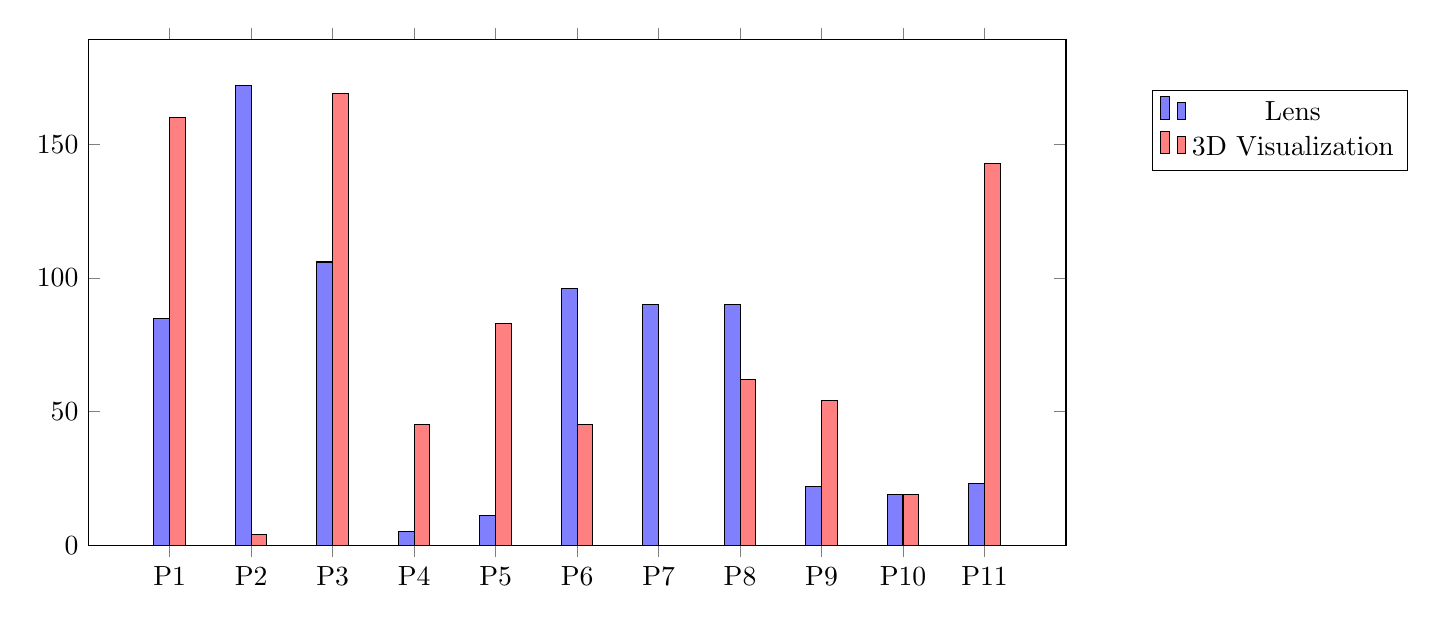
\begin{tikzpicture}
\begin{axis}[ 
    width=14cm,
    height=8cm,
    bar width=0.2cm, 
    ybar=0,
    ymin=0,
    symbolic x coords={P1, P2, P3, P4, P5, P6, P7, P8, P9, P10, P11},
    xtick=data, 
    legend style={at={(1.35, 0.9)}},
    ]
    \addplot[ybar,fill=blue!50] 
       coordinates { (P1,85) (P2,172)(P3,106) 
                     (P4,5)  (P5,11) (P6,96)
                     (P7,90) (P8,90) (P9,22)
                     (P10,19) (P11,23)
       }; 
    \addplot[ybar,fill=red!50] 
       coordinates { (P1,160) (P2,4)  (P3,169) 
                     (P4,45)  (P5,83) (P6, 45) 
                     (P7,0)   (P8,62) (P9,54)
                     (P10,19) (P11,143)
       };
    \legend{Lens, 3D Visualization}    
\end{axis}
\end{tikzpicture}
\caption{Time spent on Lens and 3D Visualization}
\label{chart:usage}     
\end{figure}
  
   
In terms of interaction within the \threed space, we observed 3 different
interaction styles. One group (P2, P7) used the lens almost exclusively
as their primary navigational tool. The second group (P4, P5, P11) were the
opposite and used direct manipulation to rotate and zoom the \threed model to
access different components. The last group used a combination of both lens
widget and direct manipulation. We also observed different behaviours, some
participants (P1, P2, P3, P11) spent a lot more time exploring the
visualization, while others (P4, P7 and P10) were more efficient in getting the
visualization to their desired orientation. A chart showing widget usage can be
seen in Figure \ref{chart:usage}.


Interaction with the heatmap widget had the most negative reactions. 4
participants thought the heatmap widget provided too much detail, they argued
that an ordinary consumer would not care for trend details, they would only care
about the overall verdict of whether a component is reliable or not. 3 other
participants had concerns about the readability of the heatmap itself, they
mentioned that the lack of labelling makes it difficult to identify individual
month, also the additional colour encoding that is applied to the border of each
cell in comparison mode made it more difficult to distinguish the different
severity levels. Participants liked using the lens to focus on specific
objects, particularly for revealing entities that were unknown to them
before. Several participants tried to use the lens' depth function to access
occluded objects, however we observed that there were difficulties making fine
adjustments, especially if the objects are located within close proximity to each other.
  
Overall, the receptions of using the visualization system were positive;
comments such as ``cool,'' ``relatable,'' and ``that was really neat'' were heard
through out the study sessions. Other comments, such as ``seeing all the different angles is
nice'' and ``even though there are some interaction problems, it just looks
really good!'' suggested the aesthetic value in showing a non photorealistic \threed
representation.  
  